\subsection*{Performance Metrics}
Entropy: $H=-\sum_{i=1}^{n}p_i\log p_i$\\
MSE: $\frac{1}{N}\|I-\hat{I}\|^2$\\
RMSE: $\frac{\|I-\hat{I}||^2}{\|I\|^2}$\\
Signal-to-Noise: $SNR=10\log_{10}(\frac{\|I\|^2}{\|I-\hat{I}\|^2})$\\
Compression Ratio(CR):\\
$\frac{size\ of\ the\ uncompressed\ data\ (in\ bits)}{size\ of\ the\ coded\ bitstream\ (in\ bits)}$\\
Bit rate: {\color{myblue}Average number of bits per original data element after Compression}\\

\subsection*{Lossless Compression}
Huffman:
\begin{enumerate}
    \item Create nodes for all $a_i$
    \item While two or more uncombined nodes do 
    \begin{itemize}
        \item Select 2 uncombined nodes $a$ and $b$ of minimum probabilities
        \item Create a new node c of prob $P_a+P_b$, and make $a$ and $b$ children of $c$
    \end{itemize}
    \item Label the tree edges: left 0, right 1
\end{enumerate}
Birate of Huffman codes:\\
$\frac{|bitstream|}{\text{num of symbols in input}}$\\
The prefix property: {\color{myblue}no codeword is a prefix of another codeword}\\
Block-Huffman coding: {\color{myblue}Treat every block as a symbol}\\\\
RLE: $(a,L)$\\\\
Golomb:
\begin{itemize}
    \item Golomb runs $0^i1$
    \item last Golomb run may not have a tail bit
    \item parameter m's optimal value is the nearest power of $2^{p\times \frac{Ln2}{1-p}}$
    \item $p$ is the probability of the more probable bit in the input stream
    \item $Ln2=0.6931$
    \item Break input into runs of the form $0^i1$
    \item Code each Golomb run $0^i1$ as $1^q0y\ (i=qm+r)$
    \item $y$ is the binary representation of $r$, using $\log m$ bits
    \item final coded bitstream is $MPB\ code_1\ \cdots\ code_n\ tail?$
\end{itemize}
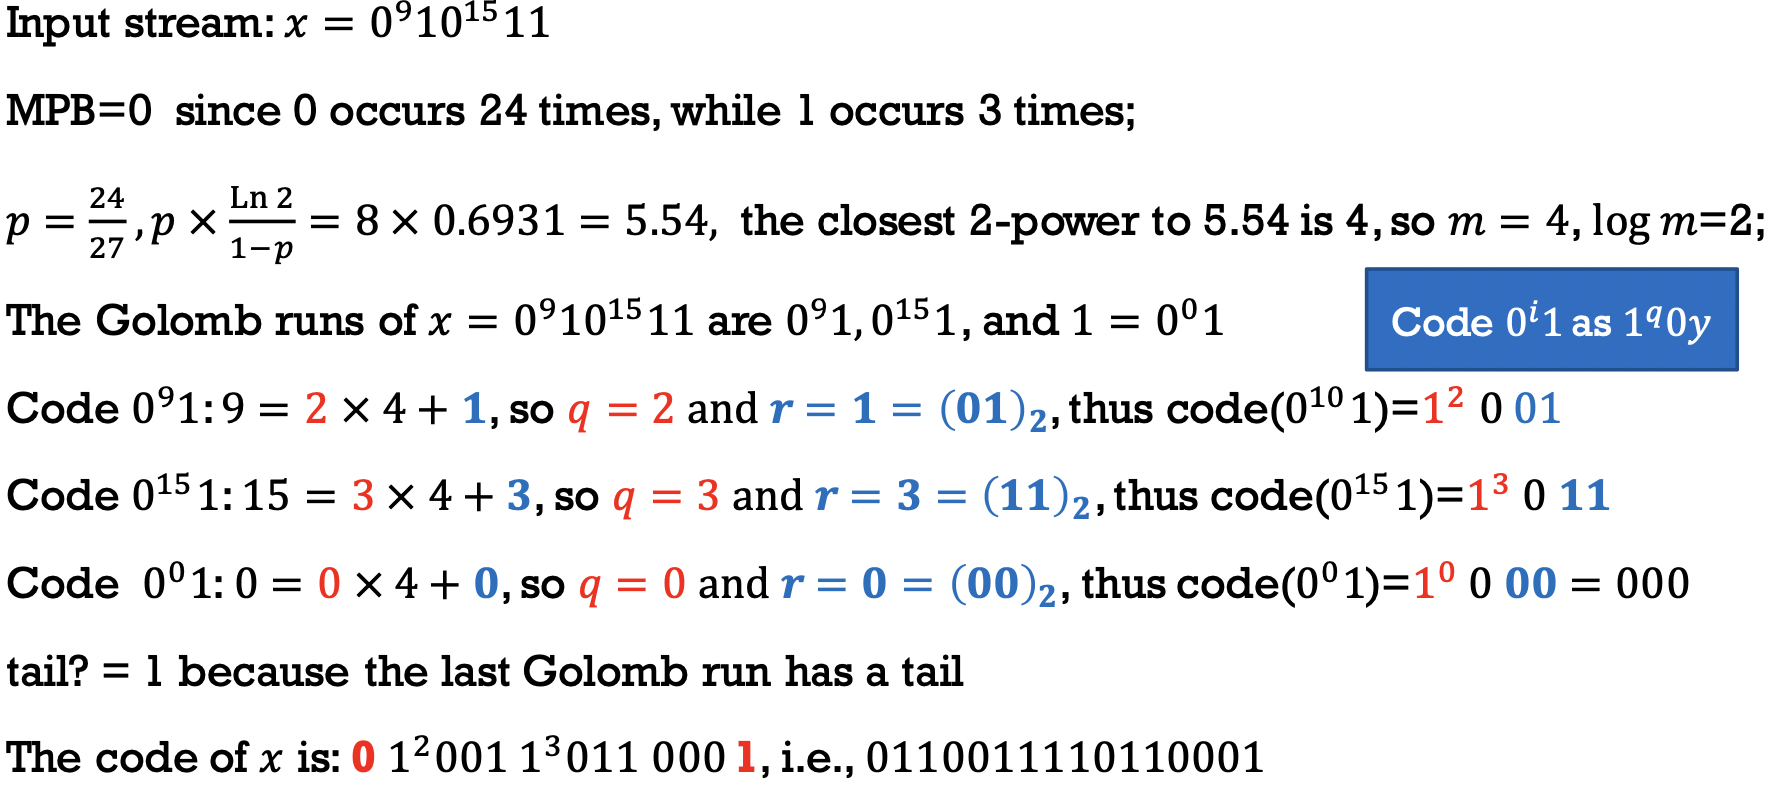
\includegraphics[width=\columnwidth]{golomb_example.png}

Differential Golomb:
\begin{enumerate}
    \item Transform $x$ to $z=z_1\cdots z_n$ where $z_i=x_i-x_{i-1}\ \forall i>1,\ and z_1=x_1$
    \item Delete the alternating negatives of the tails, we get $z'=z_1'\cdots z_n'$
    \item Code $z'$ using Golomb coding
\end{enumerate}

Arithmetic Coding:
\begin{enumerate}
    \item Let $I=[L,R)$ where initially $L=0,R=1$
    \item For $i=1$ to n do
    \begin{enumerate}
        \item Let $P_i=\Pr[0/x_1x_2\cdots x_{i-1}]$
        \item let $\Delta=R-L$
        \item If $x_i==0$ reduce $I$ to $[L,L+P_i\Delta)$
        \item Else reduce $I$ to $[L+P_i\Delta,R)$
    \end{enumerate}
    \item let $t=\lceil -\log (R-L) \rceil $, and express $\frac{L+R}{2}$ in binary as $0.r_1r_2\cdots r_t$
    \item output $0.r_1r_2\cdots r_t$
\end{enumerate}

Lempel-Ziv: 
\begin{enumerate}
    \item Set $i=1$, $J=empty$, $W=empty$, $a=x_1$, $DICT[1]=Wa(i.e.,x_1)$, output=$x_1$
    \item Set $i=2$
    \item While (there are still input symbols) do
    \begin{enumerate}
        \item Read from the remaining input until the string scanned is no longer in DICT
        \item Call that string $Wa$, where $W$ is in $DICT$ and $a$ is the input symbol after $W$
        \item Let $j$ be the index where $W=DICT[j]$
        \item Let $J=d2b(j)$ using $\lceil \log i \rceil$ bits
        \item Code $Wa$ as $(J,a)$ and append that code to the output
        \item Store $Wa$ in $DICT[i]$, i.e. $DICT[i]=Wa$
        \item i++
    \end{enumerate}
\end{enumerate}

DPCM:
\begin{enumerate}
    \item $e_1=x_1,e_i=x_i-ax_{i-1}\ \forall i\le2$
    \item Code the residuals with Huffman
    \item Let $E(a)=\sum^n_{i=1}e_i^2=\sum^n_{i=1}(x_i-ax_{i-1})^2$, assuming $x_0=0$
    \item Setting $E'(a)=0$, we get $a=\frac{\sum^n_{i=1}x_{i-1}x_i}{\sum^n_{i=1}x^2_{i-1}}$
\end{enumerate}

Gray Code: a sequence of up to $2^n$ binary strings of $n$ bits each, where 
every two successive strings \emph{differ by only one bit}
\begin{enumerate}
    \item Takes the strings of $G_{n-1}$, and append a 0 to the left of each string
    \item Take a copy of $G_{n-1}$ in reverse order, as $G^R_{n-1}$
    \item Append a 1 to the left of every string of $G^R_{n-1}$, as $1G^R_{n-1}$ 
    \item $G_n=0G_{n-1},1G^R_{n-1}$
\end{enumerate}

\subsection*{Lossy Compression}
\subsubsection*{Quantization}
General Scheme of Lossy Compression:\\
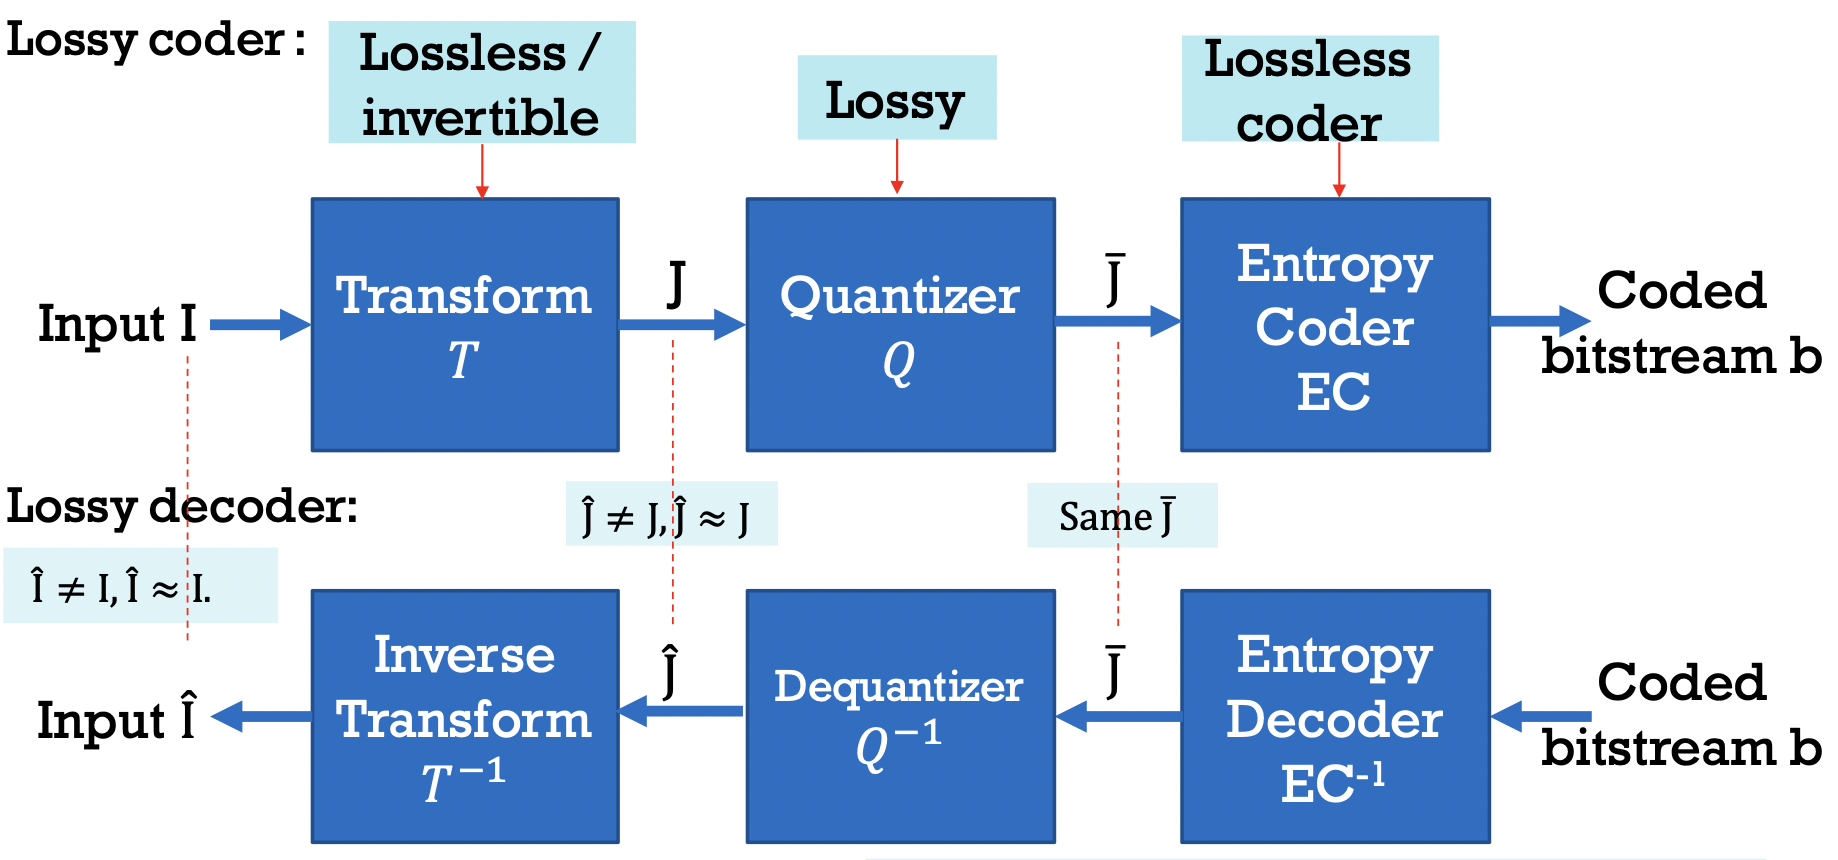
\includegraphics[width=\columnwidth]{General Scheme of Lossy Compression.png}

Scalar Quantization:\\
An $n$ level quantizer $Q$ is characterized by $n+1$
\emph{decision levels} $d_0,d_1,\cdots,d_n$, and by $n$ \emph{reconstruction levels}
$r_0,r_1,\cdots,r_{n-1}$\\\\
The quantizer $Q$ is a function that maps any real number $x\in [d_0 d_n)$ into
the unique integer $i\in {0,1,2,\cdots,n}$ such that $x\in [d_i d_{i+1})$\\\\
The dequantizer $Q^{-1}$ is a mapping from ${0,1,2,\cdots,n}$ to ${r_0,r_1,\cdots,r_{n-1}}$ where
$Q^{-1}(i)=r_i\forall i$\\

Uniform Quantizer:
\begin{itemize}
    \item $d_1-d_0=d_2-d_1=d_3-d_2=\cdots$
    \item reconstruction values are the mid-points of their intervals
    \item $\Delta=\frac{d_n-d_0}{n}$
    \item $d_i=d_0+i\Delta\ \ \forall i=1,2,\cdots,n$
    \item $r_i=\frac{d_i+d_{i+1}}{2}=d_i+\frac{\Delta}{2}=d_0+(i+\frac{1}{2})\Delta$
    \item $Q(x)=\lfloor \frac{x-d_0}{\Delta}\rfloor$
    \item $Q^{-1}(i)=d_0+(i+\frac{1}{2})\Delta$
\end{itemize}

Non-Uniform Quantizer:
\begin{itemize}
    \item the decision intervals are NOT of equal size $OR$
    \item the reconstruction levels are not all the centers of their intervals
\end{itemize}

Semi-Uniform Quantizer:
\begin{itemize}
    \item the decision intervals are ALL of equal size $AND$
    \item the reconstruction levels are not all the midpoints of their intervals
\end{itemize}

Max-Lloyd quantizer:
\begin{enumerate}
    \item Initialize $d_1,d_2,\cdots,d_{n}$ and $r_1,r_2,\cdots,r_{n-1}$ to some random values
    \item Repeat \begin{itemize}
        \item For all $i$, compute $r_i=$ the average value of the data that happen to fall in interval $[d_i\ d_{i+1}]$
        \item For all $i$, compute $d_i=\frac{r_{i+1}+r_i}{2}$
    \end{itemize}
    \item Until the error < a set tolerance
\end{enumerate}

\subsubsection*{Transform}
1D transform: $y=Ax,\ O(N^2)$\\
2D transform: $Y=A_NXA_M^T,\ O(N^3)$\\
$a_{kl}$: the $k^{th}$ row and $l^{th}$ column position of $A_N$\\

Discrete Fourier Transform: $a_{kl}=\sqrt{\frac{1}{N}}e^{-\frac{2\pi i}{N}kl}$

Discrete Cosine Transform:
\begin{itemize}
    \item $a_{0l}=\sqrt{\frac{1}{N}},\ \forall l=0,1,\cdots,N-1$
    \item $a_{kl}=\sqrt{\frac{2}{N}}\cos\frac{(l+\frac{1}{2})k\pi}{N},\ \forall k=1,2,\cdots,N-1,\ and\ l=0,1,\cdots, N-1$
    \item $A_N^{-1}=A_N^T$
\end{itemize}

Hadamard Transform:
\begin{itemize}
    \item express $k$ and $l$ in binary
    \item $a_{kl}=\sqrt{\frac{1}{N}}(-1)^{k_{n-1}l_{n-1}+\cdots+k_1l_1+k_0l_0}$
    \item $A_N^{-1}=A_N^T=A_N$
\end{itemize}

Walsh Transform:
\begin{itemize}
    \item $a_{kl}=\sqrt{\frac{1}{N}}(-1)^{k_{n-1}l_{0}+\cdots+k_1l_{n-2}+k_0l_{n-1}}$
    \item $A_N^{-1}=A_N^T=A_N$
\end{itemize}

Haar Transform:
\begin{itemize}
    \item $a_{0l}=\sqrt{\frac{1}{N}}$
    \item TODO
\end{itemize}

\subsubsection*{Complex Numbers}
$z=a+ib$\\
$re^{i\theta}=r\cos\theta+ir\sin\theta$\\
$a=r\cos\theta,b=r\sin\theta$\\
$r=\sqrt{a^2+b^2}$\\
$\frac{b}{a}=\frac{r\sin\theta}{r\cos\theta}=\frac{\sin\theta}{\cos\theta}=\tan\theta$\\
$re^{i\theta}\cdot r'e^{i\theta'}=rr'e^{i(\theta\theta')}$

\subsubsection*{Vector Spaces}
Vector space $(V,+,.,O)$:
\begin{enumerate}
    \item $\forall u,v \in V, u+v=v+u$
    \item $\forall u,v,w \in V, (u+v)+w=u+(v+w)$
    \item $\exists O \in V\ \text{such that}\ \forall u \in V, u+O=O+u=u$
    \item $\forall u \in V,\exists v \in V \text{ such that } u+v=v+u=O$
    \item $\forall a\in\mathbb{R} \text{ and }\forall u,v \in V, a(u+v)=au+av$
    \item $\forall a,b \in\mathbb{R} \text{ and }\forall u\in V,(a+b)u=au+bu$
    \item $\forall a,b \in\mathbb{R} \text{ and }\forall u\in V,a(bu)=(ab)u$
    \item $\forall u\in V,0u=O, \text{ and }1u=u$
\end{enumerate}

Linear independent:\\
If $x_1v_1+x_2v_2+,\cdots,+x_nv_n=0$\\
then we must have $x_1=x_2=\cdots=x_n=0$\\

Basis:
\begin{itemize}
    \item $v_1,v_2,\cdots,v_n$ are linearly independent
    \item $\forall v\in V$, $v$ can be expressed as a linear combination of $v_1, v_2, \cdots, v_n$
\end{itemize}

For human eyes and ears, the low-frequency contents are more important than highfrequency contents.\\